\chapter{Resultados computacionales}
\label{chap:resultados}

Este capítulo explora computacionalmente el comportamiento de PINNs en problemas de dificultad creciente. Los experimentos no constituyen una demostración de los resultados asintóticos del Capítulo~\ref{chap:convergencia}; su función es examinar, en configuraciones finitas, la relación entre pérdida empírica, residuo continuo y error respecto de una solución de referencia.

Se consideran: (i) un ejemplo elemental de regresión; (ii) una EDO logística; (iii) problemas de Poisson 1D con y sin observaciones interiores; (iv) una comparación entre PINN estándar, penalización cuadrática media y regularización Lipschitz (LIPR); (v) la reproducción de los dos experimentos elípticos unidimensionales de Shin et al.~\cite{shin2020convergence}; (vi) un experimento de diagnóstico de la regularidad H\"older para interpretar los resultados del Capítulo~\ref{chap:convergencia}; y (vii) Poisson 2D, con un análisis de estabilidad sobre mallas de prueba y un barrido de condiciones de Dirichlet fuertes y penalizadas; (viii) un estudio de la aproximación con redes $\tanh$ mediante tres protocolos A--C; y (ix) una comparación exploratoria con FEM y FVM.

\section*{Alcance y criterios de comparación}

Los métodos clásicos de malla y las PINNs resuelven el problema mediante mecanismos diferentes. FEM y FVM discretizan el operador y producen un sistema algebraico; una PINN parametriza la solución y resuelve un problema de optimización no convexo. En consecuencia, una comparación responsable debe distinguir precisión, costo, grados de libertad, número de evaluaciones del residuo y variabilidad entre entrenamientos. Las dificultades de optimización de las PINNs, incluidas las patologías de gradiente y los problemas de condicionamiento, han sido estudiadas por Wang, Teng y Perdikaris~\cite{wang2021gradient} y Krishnapriyan et al.~\cite{krishnapriyan2021failure}; los mecanismos descritos en esos trabajos no se presuponen demostrados en los experimentos de esta tesis.

En este capítulo se reportan errores relativos
\[
e_{L^2}
=
\frac{\|u_\theta-u^\star\|_{L^2(U)}}{\|u^\star\|_{L^2(U)}},
\qquad
e_{H^1}
=
\frac{\|u_\theta-u^\star\|_{H^1(U)}}{\|u^\star\|_{H^1(U)}},
\]
cuando la solución exacta $u^\star$ está disponible. 

Los códigos completos de los experimentos se presentan en el Apéndice~\ref{app:codigo},
donde también se indica el repositorio del cuaderno computacional. Los entrenamientos pueden variar
con la inicialización y el entorno de cálculo; por ello se registran sus parámetros y resultados.

\paragraph{Tres niveles de validación.}
Distinguimos (a) el ajuste de los residuos en los puntos de colocación, (b) la evaluación de los residuos y sus variaciones en una malla independiente, y (c) el error de la solución respecto de $u^\star$. El descenso de la función de pérdida por épocas se presenta en escala semilogarítmica; el error frente al número de muestras o al refinamiento, en escala log--log; las curvas de solución y superficies se representan en escala lineal. Las pérdidas de métodos diferentes no son directamente comparables cuando incluyen regularizadores distintos.

Para reproducir las gráficas de Shin es preciso distinguir también los errores \emph{RMS discretos no relativos} respecto de una malla fija $Q_K=\{z_k\}_{k=1}^K$,
\begin{align*}
E_{L^2,K}(h)&=\left(\frac1K\sum_{k=1}^{K}|h(z_k)-u^\star(z_k)|^2\right)^{1/2},\\
E_{H^1,K}(h)&=\left(E_{L^2,K}(h)^2+
\frac1K\sum_{k=1}^{K}|h'(z_k)-(u^\star)'(z_k)|^2\right)^{1/2}.
\end{align*}
Estas magnitudes son medias cuadráticas discretas (con factor $1/K$) sin normalizar por la norma de $u^\star$. Se distinguen de los errores relativos $e_{L^2}$ y $e_{H^1}$ usados en las comparaciones propias. Los valores de ambas convenciones no deben intercambiarse al contrastar las pendientes con las figuras del artículo.


\paragraph{Arquitecturas y condiciones de los ensayos.}
Las configuraciones no comparten una única familia de redes. La Tabla~\ref{tab:arquitecturas_computacionales} distingue las arquitecturas y evita interpretar las diferencias de error exclusivamente como un efecto de regularización o muestreo. Todas las configuraciones indicadas utilizan activación $\tanh$ en sus capas ocultas.
\begin{table}[htbp]
\centering
\caption{Arquitecturas de los principales experimentos. Las capas enumeradas corresponden a anchos ocultos; el tratamiento de frontera se indica por separado.}
\label{tab:arquitecturas_computacionales}
\small
\begin{tabular}{p{0.39\linewidth}p{0.27\linewidth}p{0.23\linewidth}}
\hline
Experimento & Arquitectura & Frontera \\
\hline
Regularizaciones Poisson 1D & MLP $50$--$50$ & Penalizada \\
Reproducciones 1D de Shin & Residual $50$--$50$ & Débil (tanh) o fuerte (oscilatorio) \\
Poisson 2D con observaciones & MLP $40$--$80$--$40$ & Penalizada \\
Poisson 2D sin observaciones & MLP $50$--$50$ & Penalizada \\
Barrido Poisson 2D revisado & MLP $50$--$50$ & Penalizada o fuerte \\
\hline
\end{tabular}
\end{table}

\section{Caso base: redes neuronales para estimación (regresión)}
\label{sec:regresion}

Este caso base ilustra el mecanismo de optimización por MSE que posteriormente se reutiliza en las PINNs. 

\paragraph{Problema.} Dado un conjunto de puntos $(x_i,y_i)$, aproximar una función $f(x)$ tal que $\text{NN}(x) \approx y$.

\paragraph{Implementación.} La lógica de entrenamiento para este regresor simple se describe en el Algoritmo \ref{alg:regresion}. La implementación completa en PyTorch se encuentra disponible en el Código A.1 (Apéndice A).

\begin{algorithm}
\caption{Entrenamiento de Red Neuronal para Regresión}
\label{alg:regresion}
\begin{algorithmic}[1]
\Require Datos de entrenamiento $\{(x_i, y_i)\}_{i=1}^N$, Tasa de aprendizaje $\eta$, Épocas $E$
\Ensure Parámetros óptimos de la red $\theta^*$
\State Inicializar red neuronal $\text{NN}_\theta$ (arquitectura: Linear-Tanh-Linear...)
\State Inicializar optimizador (por ejemplo, Adam)
\For{$epoch \gets 1,\ldots,E$}
    \State $\hat{y} \gets \text{NN}_\theta(x_{train})$ \Comment{Propagación hacia delante}
    \State $Loss \gets \frac{1}{N} \sum (\hat{y} - y_{train})^2$ \Comment{Cálculo de MSE}
    \State Calcular gradientes $\nabla_\theta Loss$ \Comment{Retropropagación}
    \State Actualizar $\theta \gets \theta - \eta \nabla_\theta Loss$ \Comment{Paso de optimización}
\EndFor
\State \Return $\text{NN}_{\theta^*}$
\end{algorithmic}
\end{algorithm}

Al ejecutar el algoritmo sobre el conjunto de datos sintético, obtenemos la aproximación visualizada en la Figura \ref{fig:regresion_plot}.

\begin{figure}[h!]
    \centering
    \includegraphics[width=0.9\linewidth]{imagenes/imagen2.png}
    \caption{Gráfica de la aproximación usando Redes Neuronales para regresión simple.}
    \label{fig:regresion_plot}
\end{figure}

\subsection*{Estructura mínima de una PINN}
Una PINN reutiliza la arquitectura anterior, calcula derivadas mediante diferenciación automática y minimiza una pérdida compuesta:
\[
\mathcal{J}(\theta)
=
\mathcal{J}_{\mathrm{PDE}}
+
\lambda_{\mathrm{BC}}\mathcal{J}_{\mathrm{BC}}
+
\lambda_{\mathrm{data}}\mathcal{J}_{\mathrm{data}}.
\]
Esta formulación permite combinar ecuaciones y observaciones en un mismo objetivo. Sin embargo, los pesos relativos, el muestreo y la dinámica de optimización condicionan el resultado. El método no requiere conectividad de malla, aunque sí una discretización mediante puntos de colocación.

\section{Ejemplo I: crecimiento poblacional (EDO)}
\label{sec:logistica}

\paragraph{Ecuación.} Modelamos el crecimiento poblacional mediante la ecuación logística:
\[
\frac{d f(t)}{d t}=Rf(t)(1-f(t)), \qquad f(0)=0.5.
\]
donde $R$ es la tasa máxima de crecimiento.

\paragraph{Lógica de la PINN.} La red neuronal debe minimizar el residuo de la EDO. A diferencia de la regresión simple, aquí la "etiqueta" no es un dato, sino el cumplimiento de la ecuación diferencial. El flujo de información se detalla en la Figura \ref{fig:flowchart_logistic}; su implementación figura en el Código A.2 del Apéndice A.

\begin{figure}[h!]
\centering
\begin{tikzpicture}[node distance=1.5cm, auto]
    % Nodes
    \node (input) [draw, circle, minimum size=1cm] {$t$};
    \node (nn) [draw, rectangle, rounded corners, minimum width=2.5cm, minimum height=1cm, right=of input] {NN$_\theta(t)$};
    \node (output) [draw, circle, minimum size=1cm, right=of nn] {$\hat{f}(t)$};
    
    \node (grad) [draw, rectangle, below=of output] {Autograd $\frac{d\hat{f}}{dt}$};
    \node (residual) [draw, diamond, aspect=2, below=of grad] {Residuo $r(t)$};
    \node (loss) [draw, rectangle, dashed, left=of residual] {$\mathcal{L} = \mathcal{L}_{PDE} + \mathcal{L}_{BC}$};
    \node (optim) [draw, rectangle, rounded corners, above=of loss] {Optimizador};

    % Arrows
    \draw[->] (input) -- (nn);
    \draw[->] (nn) -- (output);
    \draw[->] (output) -- (grad);
    \draw[->] (grad) -- (residual);
    \draw[->] (output) to[bend left=45] (residual); % Connection for f(t) in residual
    \draw[->] (residual) -- (loss);
    \draw[->] (loss) -- (optim);
    \draw[->] (optim) -- (nn);
    
    % Labels
    \node[right=0.1cm of residual, font=\footnotesize] {$r = \frac{d\hat{f}}{dt} - R\hat{f}(1-\hat{f})$};
\end{tikzpicture}
\caption{Diagrama de flujo para el entrenamiento de la PINN en la ecuación logística.}
\label{fig:flowchart_logistic}
\end{figure}

Calculamos una solución numérica de referencia y la comparamos con la salida de la PINN. En la configuración mostrada en la Figura~\ref{fig:logistic_comparison}, ambas curvas presentan una concordancia visual alta. El valor de error reportado corresponde a esta ejecución y no debe interpretarse como una garantía independiente de la inicialización o del optimizador.

\begin{figure}[h!]
    \centering
    \includegraphics[width=0.9\linewidth]{imagenes/comparison.png}
    \caption{Gráfica de la comparación entre la NN y la solución numérica.}
    \label{fig:logistic_comparison}
\end{figure}

\begin{figure}[htbp]
    \centering
    \includegraphics[width=0.92\linewidth]{imagenes/solucion_y_componentes_logistica.png}
    \caption{Ecuación logística: comparación de soluciones y evolución semilogarítmica de la pérdida total, el residuo diferencial, la condición inicial y las observaciones. Las componentes corresponden a la función objetivo, no a una descomposición del error respecto de la solución exacta.}
    \label{fig:logistica_perdidas}
\end{figure}

En esta ejecución la pérdida total descendió desde $2.15\times10^{-1}$ hasta valores del orden de $10^{-5}$, con $2\,000$ épocas de Adam. La solución de referencia se obtuvo numéricamente con \texttt{solve\_ivp}. El desglose permite identificar qué restricciones se satisfacen antes y cuáles requieren más entrenamiento, sin atribuir a cada término una fracción del error funcional.

\section{Poisson 1D (EDO de segundo orden)}
\label{sec:poisson1d}
Para $u_{xx}(x)=-\pi^2\sin(\pi x)$ en $[-1,1]$ con $u(\pm1)=0$, esperamos que la PINN aprenda $u^\star(x)=\sin(\pi x)$.

\subsection{Ejemplo II: Poisson 1D con datos escasos}
La PINN impone el residuo $r(x)=u_{xx}+\pi^2\sin(\pi x)$ junto con las condiciones de Dirichlet. El procedimiento computacional para calcular las derivadas de segundo orden necesarias para el residuo se describe en el Algoritmo \ref{alg:poisson1d}. La implementación completa se encuentra en el Código A.3 (Apéndice A).

\begin{algorithm}
\caption{Cálculo de Pérdida para Poisson 1D}
\label{alg:poisson1d}
\begin{algorithmic}[1]
\Function{CalcularPerdida}{$\text{NN}_\theta, x_{col}, x_{bc}, x_{data}, y_{data}$}
    \State $u \gets \text{NN}_\theta(x_{col})$
    \State $u_x \gets \nabla_x u$ \Comment{Primera derivada (Autograd)}
    \State $u_{xx} \gets \nabla_x u_x$ \Comment{Segunda derivada (Autograd)}
    
    \State $f_{source} \gets -\pi^2 \sin(\pi x_{col})$
    \State $\mathcal{L}_{PDE} \gets \text{Mean}((u_{xx} - f_{source})^2)$
    
    \State $\mathcal{L}_{BC} \gets \text{Mean}((\text{NN}_\theta(x_{bc}) - 0)^2)$
    \State $\mathcal{L}_{Data} \gets \text{Mean}((\text{NN}_\theta(x_{data}) - y_{data})^2)$
    
    \State \Return $\mathcal{L}_{PDE} + \mathcal{L}_{BC} + \mathcal{L}_{Data}$
\EndFunction
\end{algorithmic}
\end{algorithm}

La convergencia de los componentes de la función de pérdida se muestra a continuación.

\begin{figure}[h!]
    \centering
    \includegraphics[width=0.9\linewidth]{imagenes/convergence.png}
    \caption{Gráfica de la convergencia de la función de pérdida y sus componentes.}
    \label{fig:poisson1d_conv}
\end{figure}

\begin{figure}[htbp]
\centering
\includegraphics[width=0.90\linewidth]{imagenes/solucion_y_componentes_poisson_seno.png}
\caption{Poisson 1D con datos escasos: solución exacta y aproximación neuronal (escala lineal), seguidas de la pérdida total y sus componentes (escala semilogarítmica).}
\label{fig:poisson_seno_desglose}
\end{figure}

La pérdida inicial fue cercana a $47.76$ y, después de $5\,000$ épocas, alcanzó aproximadamente $2.7\times10^{-4}$. La mayor contribución al comienzo corresponde al residuo de la ecuación. La concordancia visual de las soluciones debe interpretarse junto a esta evolución, no en reemplazo de ella.

\subsection{Ejemplo III: Ecuación de Poisson 1D con datos de observación}
En este caso, resolvemos $\frac{\partial^2 u}{\partial x^2} = -2 \text{Sech}^2(x)\text{Tanh}(x)$ con condiciones de frontera tipo Tanh. La estructura algorítmica es análoga al caso anterior, modificando únicamente la función fuente y los datos de borde. La implementación se detalla en el Código A.4 (Apéndice A).

\begin{figure}[h!]
    \centering
    \includegraphics[width=0.9\linewidth]{imagenes/comparison3_data.png}
    \caption{Comparación entre PINN y solución analítica con datos observados.}
    \label{fig:poisson_data}
\end{figure}

\begin{figure}[htbp]
\centering
\includegraphics[width=0.90\linewidth]{imagenes/solucion_y_componentes_poisson_tanh_con_datos.png}
\caption{Poisson 1D con observaciones: comparación de soluciones y descomposición semilogarítmica de las pérdidas residual, de frontera y de datos.}
\label{fig:poisson_tanh_datos_desglose}
\end{figure}

En la ejecución representada, la pérdida total disminuye varios órdenes de magnitud y los errores relativos $L^2$ y $H^1$ son pequeños. La pérdida de entrenamiento y el error funcional no son cantidades equivalentes; por ello, ambos deben reportarse por separado junto con el conjunto de evaluación utilizado.

\subsection{Ejemplo IV: Ecuación de Poisson 1D sin datos de observación}
Este experimento muestra que, para el problema considerado, puede obtenerse una aproximación sin observaciones interiores, utilizando únicamente el residuo diferencial y las condiciones de frontera. No se concluye que la ecuación sea siempre un regularizador suficiente: la identificabilidad y la estabilidad dependen del problema y de las condiciones auxiliares. La pérdida se reduce a $\mathcal{J}=\mathcal{J}_{\mathrm{PDE}}+\mathcal{J}_{\mathrm{BC}}$. La implementación corresponde al Código A.5 (Apéndice A).

\begin{figure}[h!]
    \centering
    \includegraphics[width=0.9\linewidth]{imagenes/comparison4_wdata.png}
    \caption{Comparación entre PINN y solución analítica sin datos de observación.}
    \label{fig:poisson_nodata}
\end{figure}

\begin{figure}[htbp]
\centering
\includegraphics[width=0.90\linewidth]{imagenes/solucion_y_componentes_poisson_tanh_sin_datos.png}
\caption{Poisson 1D sin observaciones interiores: solución analítica y PINN, y evolución de las pérdidas residual y de Dirichlet.}
\label{fig:poisson_tanh_sin_datos_desglose}
\end{figure}

Para esta ejecución se obtuvieron los errores relativos $e_{L^2}=2.88\times10^{-5}$ y $e_{H^1}=8.58\times10^{-5}$ después de $5\,000$ épocas. Estos valores se calcularon sobre un conjunto de evaluación diferente de los puntos utilizados para minimizar la pérdida. El experimento muestra que el residuo y la frontera pueden bastar para aproximar la solución de este problema; no prueba que añadir observaciones sea siempre innecesario.

\subsection{PINN estándar, regularización cuadrática media y LIPR}
\label{subsec:regularizacion_1d}

\paragraph{Problema de referencia.}
Retomamos la ecuación de Poisson en $I=(-1,1)$,
\[
\begin{aligned}
-u''(x)&=f(x),\qquad u^\star(x)=\tanh(x),\\
u(-1)&=\tanh(-1),\qquad u(1)=\tanh(1).
\end{aligned}
\]
con $f(x)=2\tanh(x)\operatorname{sech}^2(x)$. Este problema permite comparar la PINN estándar con dos penalizaciones diferentes de la tercera derivada. El término ``LIPR'' se reserva, de aquí en adelante, para el funcional discreto utilizado por Shin et al.~\cite{shin2020convergence}, ecuación (4.1) de su artículo.

\paragraph{Estrategia de regularización.}
Dado $T_r=\{x_i\}_{i=1}^{N_f}$ y $T_b=\{-1,1\}$, definimos el residuo
$r_\theta=-u_\theta''-f$ y la pérdida base
\[
\mathcal J_{\mathrm{PINN}}(\theta)
=\frac1{N_f}\sum_{i=1}^{N_f}|r_\theta(x_i)|^2
+\lambda_b\,\frac{|u_\theta(-1)-u^\star(-1)|^2+|u_\theta(1)-u^\star(1)|^2}{2}.
\]
La penalización cuadrática \emph{media} utilizada como comparación adicional es
\[
\mathcal R_{\mathrm{media}}(\theta)
=\frac1{N_f}\sum_{i=1}^{N_f}|u_\theta'''(x_i)|^2,
\qquad
\mathcal J_{\mathrm{media}}=\mathcal J_{\mathrm{PINN}}
+\lambda_{r,N_f}^{R}\mathcal R_{\mathrm{media}}.
\]
La regularización \emph{LIPR} discreta del artículo, en cambio, penaliza el máximo de la derivada del operador $\mathcal L[u]=-u''$:
\begin{align*}
\mathcal R_{\mathrm{LIPR}}(\theta)
&=\max_{1\leq i\leq N_f}|\partial_x\mathcal L[u_\theta](x_i)|^2
=\max_{1\leq i\leq N_f}|u_\theta'''(x_i)|^2,\\
\mathcal J_{\mathrm{LIPR}}
&=\mathcal J_{\mathrm{PINN}}+\lambda_{r,N_f}^{R}\mathcal R_{\mathrm{LIPR}}.
\end{align*}
La diferencia entre media y máximo es sustancial: la segunda penalización responde al mayor valor de la derivada observado en los puntos de entrenamiento. Para la comparación con la primera figura de Shin tomamos $\lambda_b=1$ y $\lambda_{r,N_f}^{R}=N_f^{-3/2}$. Estas pérdidas \emph{discretas} no son la seminorma H\"older \emph{continua} usada en los teoremas del Capítulo~\ref{chap:convergencia}.

\begin{algorithm}
\caption{Cálculo de las tres pérdidas para Poisson 1D}
\label{alg:lipr}
\begin{algorithmic}[1]
\Require Red $u_\theta$, puntos $T_r$, extremos $T_b$, pesos $\lambda_b,\lambda_{r,N_f}^{R}$
\State Calcular $u_{xx}$ y $u_{xxx}$ mediante diferenciación automática
\State $\mathcal J_{\mathrm{PDE}}\gets \operatorname{Mean}((-u_{xx}-f(T_r))^2)$
\State $\mathcal J_{\mathrm{BC}}\gets \operatorname{Mean}((u_\theta(T_b)-g(T_b))^2)$
\State $\mathcal J_{\mathrm{PINN}}\gets\mathcal J_{\mathrm{PDE}}+\lambda_b\mathcal J_{\mathrm{BC}}$
\State $\mathcal R_{\mathrm{media}}\gets\operatorname{Mean}(u_{xxx}^2)$ \Comment{Suavidad promedio}
\State $\mathcal R_{\mathrm{LIPR}}\gets\operatorname{Max}(u_{xxx}^2)$ \Comment{Máximo discreto, Shin (4.1)}
\State $\mathcal J_{\mathrm{media}}\gets\mathcal J_{\mathrm{PINN}}+\lambda_{r,N_f}^{R}\mathcal R_{\mathrm{media}}$
\State $\mathcal J_{\mathrm{LIPR}}\gets\mathcal J_{\mathrm{PINN}}+\lambda_{r,N_f}^{R}\mathcal R_{\mathrm{LIPR}}$
\State \Return $\mathcal J_{\mathrm{PINN}},\mathcal J_{\mathrm{media}},\mathcal J_{\mathrm{LIPR}}$
\end{algorithmic}
\end{algorithm}

\paragraph{Comparación exploratoria.}
El barrido numérico del cuaderno implementa las tres funciones objetivo con la misma discretización y evalúa, fuera del conjunto de entrenamiento, los errores relativos $L^2$ y $H^1$. En los experimentos realizados la PINN estándar alcanza errores menores; las dos variantes regularizadas exhiben una disminución marcada de los errores al crecer $N_f$, pero no la superan en el intervalo ensayado. La interpretación debe incluir que $\lambda_{r,N_f}^{R}$ decrece a la vez que aumenta $N_f$; por tanto, las pendientes no estiman aisladamente el efecto de la densidad de colocación.

Los datos proceden de $7$ tamaños de muestra ($10\leq N_f\leq640$), tres semillas por tamaño y método, $4\,000$ épocas Adam y hasta $350$ iteraciones L--BFGS. La Tabla~\ref{tab:regularizaciones_1d} presenta una selección de las medianas obtenidas, sin confundirlas con los errores RMS discretos no relativos de la reproducción bibliográfica.

\begin{table}[htbp]
\centering
\caption{Errores relativos medianos $L^2$ en la comparación exploratoria de regularizaciones. Tres semillas por configuración.}
\label{tab:regularizaciones_1d}
\small
\begin{tabular}{rccc}
\hline
$N_f$ & PINN & Media cuadrática & LIPR--Shin \\
\hline
$10$ & $8.10\times10^{-6}$ & $1.25\times10^{-2}$ & $2.64\times10^{-2}$ \\
$40$ & $6.92\times10^{-6}$ & $2.19\times10^{-3}$ & $5.85\times10^{-3}$ \\
$160$ & $6.43\times10^{-6}$ & $2.87\times10^{-4}$ & $1.07\times10^{-3}$ \\
$640$ & $6.28\times10^{-6}$ & $3.75\times10^{-5}$ & $1.23\times10^{-4}$ \\
\hline
\end{tabular}
\end{table}

\begin{figure}[h!]
    \centering
    \includegraphics[width=0.9\linewidth]{imagenes/figura_pinn_media_lipr_1d.png}
    \caption{Errores relativos $L^2$ y $H^1$ (escala log--log) para PINN estándar, regularización cuadrática media y LIPR discreta, con la misma ecuación de Poisson 1D. Elaboración propia a partir del cuaderno computacional.}
    \label{fig:lipr_results}
\end{figure}

\begin{figure}[htbp]
\centering
\includegraphics[width=0.90\linewidth]{imagenes/desglose_perdidas_regularizacion.png}
\caption{Componentes de las funciones objetivo para PINN estándar, penalización media y LIPR. Se muestra por separado el término de regularización ponderado; las pérdidas totales de los tres modelos no representan la misma función objetivo.}
\label{fig:regularizacion_componentes}
\end{figure}

Esta comparación no es una reproducción literal de la Figura 3 de Shin: para reproducirla es necesario igualar además arquitectura, inicialización, número de épocas, definición del error y rango de tamaños de muestra. Tales condiciones se describen a continuación.

\paragraph{Interpretación de la recta de referencia en las figuras de Shin.}
Las figuras de reproducción muestran una recta visual de pendiente $-1$, rotulada $N_f^{-1}$. Su posición vertical se fija con la mediana de los errores positivos de ambas métricas y métodos, multiplicada por la media geométrica de los valores extremos de $N_f$; en términos del código, $C=\operatorname{mediana}(E_{\rm positivos})\sqrt{N_{f,\min}N_{f,\max}}$, y se dibuja $C/N_f$. Esta normalización usa los datos observados, pero no ajusta una pendiente mediante regresión ni representa una tasa teórica derivada de los teoremas.

\subsection{Reproducción del primer experimento elíptico de Shin: Dirichlet débil}
\label{subsec:shin_tanh}

\paragraph{Objetivo y condiciones del artículo.}
La Figura 3 de Shin et al.~\cite{shin2020convergence} estudia la solución $u^\star=\tanh(x)$ con $N_f$ entre $1$ y $10^4$. La implementación genera $N_f$ puntos de colocación con \texttt{linspace}, desde $-1$ hasta $1$: para $N_f\geq2$ se incluyen ambos extremos, que pertenecen a la frontera y no al abierto $(-1,1)$; para $N_f=1$ se usa el punto $0$. Por tanto, \emph{puntos de colocación en el intervalo cerrado} es aquí más exacto que \emph{puntos interiores}. Esta decisión preserva el protocolo computacional documentado, sin identificarlo con las muestras interiores i.i.d. de los teoremas. Los errores se miden en una malla de evaluación fija de $10^4$ o $5\times10^4$ puntos. Se utiliza inicialización Xavier~\cite{glorot2010understanding}, Adam seguido de L--BFGS~\cite{liunocedal1989lbfgs} y una red \emph{residual} con dos capas ocultas de 50 neuronas y activación $\tanh$. En particular, la arquitectura descrita por los autores puede expresarse como
\[
N_\theta(x)=W^3\tanh\!\left(W^2\bigl(\mathbf{1}x+\tanh(W^1x+b^1)\bigr)+b^2\right)+b^3,
\]
donde $\mathbf 1\in\mathbb R^{50}$ replica la entrada escalar. La presencia de la conexión residual y los pasos de optimización deben conservarse para estudiar una reproducción fiel, en lugar de usar únicamente una MLP convencional. Se adopta $\lambda_b=1$, $\lambda_{r,N_f}^{R}=N_f^{-3/2}$ y hasta $25\,000$ épocas de Adam con lote completo, seguidas de L--BFGS.

Aunque la ecuación (4.1) impresa en el artículo escribe el término de borde en forma homogénea, para la solución $u^\star=\tanh(x)$ se aplican necesariamente los datos no homogéneos $g(\pm1)=\tanh(\pm1)$. Este detalle se declara explícitamente para asegurar coherencia entre el problema y el entrenamiento.

\begin{algorithm}
\caption{Protocolo de reproducción del experimento de Shin con $u^\star=\tanh$}
\label{alg:shin_tanh}
\begin{algorithmic}[1]
\Require Tamaños $N_f$, semillas, arquitectura residual $N_\theta$, malla de evaluación $Q_K$
\For{cada $N_f$ y cada semilla}
    \State Generar $T_r$ equiespaciado en $[-1,1]$ (incluye extremos si $N_f\geq2$) e inicializar la red con Xavier
    \State Fijar $\lambda_b=1$ y $\lambda_{r,N_f}^{R}=N_f^{-3/2}$
    \For{cada método en $\{\mathrm{PINN},\mathrm{LIPR}\}$}
        \State Restaurar la misma inicialización para una comparación pareada
        \State Minimizar la pérdida correspondiente con Adam y luego L--BFGS
        \State Evaluar $E_{L^2,K}$ y $E_{H^1,K}$ sobre $Q_K$ \Comment{Sin normalizar}
        \State Guardar la semilla, las pérdidas, los errores y el tiempo
    \EndFor
\EndFor
\State Dibujar errores contra $N_f$ en escala log--log y contrastar con la Figura 3 de \cite{shin2020convergence}
\end{algorithmic}
\end{algorithm}

% Figura de reproducción bibliográfica: habilitar cuando exista una ejecución
% que haya seguido el protocolo de Shin (no sustituir con la figura exploratoria).
\IfFileExists{imagenes/reproduccion_shin_figura3.png}{%
\begin{figure}[h!]
    \centering
    \includegraphics[width=0.9\linewidth]{imagenes/reproduccion_shin_figura3.png}
    \caption{Reproducción del primer experimento de Poisson 1D de Shin: errores discretos $L^2$ y $H^1$ para PINN y LIPR, contrastados con la Figura 3 de \cite{shin2020convergence}.}
    \label{fig:reproduccion_shin_3}
\end{figure}
}{}

\paragraph{Resultados obtenidos.}
Se completaron $30$ entrenamientos, correspondientes a $15$ tamaños de muestra y dos métodos (PINN estándar y LIPR).
Los tamaños se tomaron del conjunto
\[
\begin{gathered}
N_f\in\{1,2,4,8,10,20,40,80,160,320,640,1280,\\
2500,5000,10000\}.
\end{gathered}
\] Cada entrenamiento utilizó $25\,000$ épocas de Adam y una etapa L--BFGS de hasta $250$ iteraciones, con errores RMS discretos no relativos sobre $10\,000$ puntos. Para $N_f=1$ los errores $L^2$ fueron $5.71\times10^{-2}$ (PINN) y $2.80\times10^{-2}$ (LIPR); para $N_f=10\,000$ descendieron a $6.95\times10^{-7}$ y $1.22\times10^{-6}$, respectivamente. En $H^1$, a $N_f=10\,000$ se obtuvieron $8.52\times10^{-6}$ y $9.15\times10^{-6}$.

La Figura~\ref{fig:reproduccion_shin_3} muestra, para LIPR, una disminución neta del error al crecer el número de puntos, con oscilaciones para algunos valores de $N_f$. La PINN estándar alcanza errores muy pequeños desde tamaños moderados; su curva no es monótona. Se reproduce así una comparación cualitativa del experimento bibliográfico, pero no cabe inferir una tasa asintótica a partir de una sola semilla ni de estas iteraciones finitas.

\subsection{Reproducción del segundo experimento elíptico de Shin: Dirichlet fuerte}
\label{subsec:shin_frontera_fuerte}

\paragraph{Problema de alta frecuencia.}
El segundo caso de Poisson 1D del artículo utiliza
\[
u^\star(x)=(1-x^2)\sin(6\pi x),\qquad
-u''(x)=f(x),\qquad u(-1)=u(1)=0,
\]
con
\[
f(x)=\bigl(2+36\pi^2(1-x^2)\bigr)\sin(6\pi x)
+24\pi x\cos(6\pi x).
\]
La condición de frontera se impone \emph{exactamente} mediante la parametrización
\[
h_\theta(x)=(1-x^2)N_\theta(x),
\quad\text{de modo que}\quad h_\theta(-1)=h_\theta(1)=0
\quad\text{para todo }\theta.
\]
Se conserva la arquitectura residual del primer ensayo. Shin considera tamaños de muestra entre $50$ y $5\,000$, regularización $\lambda_{r,N_f}^{R}=N_f^{-3/2}$, Adam durante $5\,000$ o $25\,000$ épocas, lotes de tamaño $100$ y una etapa posterior de L--BFGS. Esta prueba está especialmente vinculada con la conclusión $H^1$ del Teorema~4, pues elimina el defecto de frontera por construcción.

\begin{algorithm}
\caption{Protocolo para Poisson 1D oscilatorio con frontera fuerte}
\label{alg:shin_oscila}
\begin{algorithmic}[1]
\Require Puntos $T_r$, red residual $N_\theta$, peso $\lambda_{r,N_f}^{R}$, malla $Q_K$
\State Construir $h_\theta(x)=(1-x^2)N_\theta(x)$ \Comment{Dirichlet exacto}
\State Calcular $r_\theta(x)=-h_\theta''(x)-f(x)$ por Autograd
\For{cada método en $\{\mathrm{PINN},\mathrm{LIPR}\}$}
    \State Formar $\mathcal J_{\mathrm{PINN}}=\operatorname{Mean}(r_\theta(T_r)^2)$
    \State Para LIPR, sumar $\lambda_{r,N_f}^{R}\operatorname{Max}(h_\theta'''(T_r)^2)$
    \State Entrenar con Adam y L--BFGS según el protocolo del artículo
    \State Evaluar errores $L^2$, $H^1$ y $C^0$ en $Q_K$
\EndFor
\State Comparar las curvas log--log con la Figura 4 de \cite{shin2020convergence}
\end{algorithmic}
\end{algorithm}

% La imagen se incorpora solo al disponer de resultados efectivamente calculados.
\IfFileExists{imagenes/reproduccion_shin_figura4.png}{%
\begin{figure}[h!]
    \centering
    \includegraphics[width=0.9\linewidth]{imagenes/reproduccion_shin_figura4.png}
    \caption{Comparación con el segundo experimento de Shin: errores discretos $L^2$ y $H^1$ bajo Dirichlet fuerte. La ejecución realizada no reproduce la tendencia decreciente de referencia.}
    \label{fig:reproduccion_shin_4}
\end{figure}
}{}

\noindent En el protocolo oscilatorio se emplea la misma construcción de puntos de colocación sobre el intervalo cerrado; con $N_f=2$ ambos puntos pertenecen a la frontera, incluso cuando la condición de Dirichlet se impone exactamente.\par

\paragraph{Resultado de la reproducción oscilatoria.}
Se completaron $16$ entrenamientos, para $N_f=50,100,200,500,1000,2000,3500,5000$ y ambos métodos, con $5\,000$ épocas Adam, lotes de tamaño $100$ y una etapa L--BFGS de hasta $250$ iteraciones. La condición de Dirichlet se satisface exactamente por construcción. Sin embargo, las curvas de la Figura~\ref{fig:reproduccion_shin_4} no presentan la reducción sistemática de error buscada. Por ejemplo, en $N_f=5\,000$ los errores discretos $L^2$ son $1.780$ (PINN) y $1.815$ (LIPR), y los errores $H^1$ son $3.682$ y $7.147$, respectivamente. En $N_f=50$ la PINN alcanzó $E_{L^2}=1.60\times10^{-2}$, pero su error creció y osciló al variar el muestreo.

La satisfacción exacta de las condiciones de frontera no garantiza una aproximación precisa cuando el entrenamiento no reduce suficientemente el residuo. La discrepancia con la Figura 4 de Shin requiere examinar la optimización y la sensibilidad a sus parámetros, incluido el régimen de $25\,000$ épocas considerado por los autores. Los estudios de Wang, Teng y Perdikaris~\cite{wang2021gradient} y de Krishnapriyan et al.~\cite{krishnapriyan2021failure} ofrecen posibles explicaciones generales relacionadas con gradientes desbalanceados y condicionamiento; no identifican, por sí mismos, la causa del comportamiento registrado aquí.

\paragraph{Diagnóstico controlado posterior.}
Se identificó una inconsistencia en una implementación preliminar: el factor de
regularización $\lambda_{r,N_f}^{R}=N_f^{-3/2}$ se había calculado a partir del tamaño del lote recibido por la función de pérdida, lo que modificaba su valor al pasar de Adam a L--BFGS. El protocolo revisado fija el peso mediante el número \emph{total} $N_f$; durante Adam, el máximo LIPR sigue siendo un máximo \emph{de minilote} cuando se utiliza ese régimen, y no equivale al máximo en todos los puntos. La PINN no regularizada no depende de $\lambda_{r,N_f}^{R}$, de modo que este defecto no explica por sí solo sus errores.

En un ensayo separado se mantuvieron la semilla $2026$, $2\,500$ actualizaciones Adam y hasta $100$ iteraciones L--BFGS, con una evaluación independiente en $2\,001$ puntos. Para $N_f=200$, la PINN obtuvo errores discretos $L^2$ de $0.6630$ con lote completo y $0.2784$ con minilote $100$; LIPR obtuvo $0.3519$ y $0.8372$, respectivamente. Los resultados no respaldan una explicación única basada en el tamaño de lote. Tampoco constituyen una reproducción equivalente del régimen principal, porque el presupuesto y la malla de prueba son distintos. La Tabla~\ref{tab:shin_diagnostico_nuevo} presenta las magnitudes pertinentes.

\begin{table}[htbp]
\centering
\caption{Diagnóstico controlado del problema oscilatorio, con $N_f=200$, una semilla y dos regímenes de lote. Errores RMS discretos no normalizados.}
\label{tab:shin_diagnostico_nuevo}
\begin{tabular}{lcc}
\hline
Método & Lote completo & Minilote $100$ \\
\hline
PINN & $0.6630$ & $0.2784$ \\
LIPR & $0.3519$ & $0.8372$ \\
\hline
\end{tabular}
\end{table}

El cálculo se documenta en el Apéndice~\ref{app:protocolo_revisado}, junto con el archivo de resultados y el cuaderno completo. El caso oscilatorio permanece como discrepancia experimental no resuelta y no se interpreta como refutación de los resultados de convergencia, cuyos supuestos no se verifican automáticamente mediante entrenamiento finito.

\subsection{Interpretación computacional de la regularidad H\"older}
\label{subsec:holder_experimento}

\paragraph{Relación con la pérdida del Capítulo III.}
La regularización teórica de Shin, ecuación (3.3), emplea una seminorma continua. En dimensión uno, para $\mathcal L[u]=-u''$, el funcional relevante es
\begin{align*}
\mathcal J_{\mathrm{H}}(\theta)
&=\mathcal J_{\mathrm{PINN}}(\theta)
+\lambda_{r,N_f}^{R}[\mathcal L[h_\theta]]_{\alpha;I}^{2},\\
[v]_{\alpha;I}
&=\sup_{x\neq y\in I}\frac{|v(x)-v(y)|}{|x-y|^{\alpha}},\qquad 0<\alpha\leq1.
\end{align*}
A diferencia de LIPR, que maximiza una derivada sobre los puntos de colocación, esta expresión toma el supremo de \emph{todos} los cocientes de H\"older del operador en el dominio. Para $\alpha=1$ ambos procedimientos aproximan el mismo control Lipschitz continuo cuando la función es suficientemente regular, aunque sus objetivos discretos usan conjuntos y operaciones distintos; no son tres nociones teóricas independientes de regularización. Para $\alpha=1$, con regularidad suficiente y $I$ convexo,
\[
[\mathcal L[h_\theta]]_{1;I}
=\sup_{x\in I}|\partial_x\mathcal L[h_\theta](x)|
=\sup_{x\in I}|h_\theta'''(x)|.
\]
La sustitución del supremo continuo por un máximo en muestras finitas no es una identidad matemática; es la aproximación numérica que motiva LIPR.

Para estudiar también $\alpha\in(0,1)$ se utiliza una malla auxiliar $Q_K=\{z_1,\dots,z_K\}$, independiente de los puntos residuales, y se evalúa
\[
S_{K,\alpha}(h_\theta)
=\max_{i<j}\frac{|\mathcal L[h_\theta](z_i)-\mathcal L[h_\theta](z_j)|}
{|z_i-z_j|^\alpha}
\ \leq\ [\mathcal L[h_\theta]]_{\alpha;I}.
\]
El máximo discreto es una \emph{cota inferior} de la seminorma continua. Aumentar $K$ permite examinar su estabilidad numérica, pero no certifica haber calculado el supremo exacto. El costo de la comparación de todos los pares es $O(K^2)$ y puede reducirse mediante procesamiento por bloques.

\begin{algorithm}
\caption{Aproximación discreta del control H\"older y evaluación del residuo}
\label{alg:holder_diagnostico}
\begin{algorithmic}[1]
\Require PINN entrenada $h_\theta$, puntos de colocación $T_r$, malla de prueba $Q_K$, exponente $\alpha$
\State Evaluar $\mathcal L[h_\theta](z_k)$ y $r_\theta(z_k)=\mathcal L[h_\theta](z_k)-f(z_k)$ en $Q_K$
\State $S_{K,\alpha}\gets0$
\For{$i\gets1,\ldots,K$}
    \For{$j\gets i+1,\ldots,K$}
        \State $S_{K,\alpha}\gets\max\!\left\{S_{K,\alpha},\frac{|\mathcal L[h_\theta](z_i)-\mathcal L[h_\theta](z_j)|}{|z_i-z_j|^\alpha}\right\}$
    \EndFor
\EndFor
\State Estimar $\|r_\theta\|_{\infty,Q_K}$ y la pérdida residual media en $Q_K$
\State Calcular el radio de cobertura evaluado $\delta_{m,K}=\max_{z\in Q_K}\min_{x_i\in T_r}|z-x_i|$
\State \Return $S_{K,\alpha},\|r_\theta\|_{\infty,Q_K},\delta_{m,K}$
\end{algorithmic}
\end{algorithm}

\paragraph{Interpretación del lema de cobertura.}
Con $r_\theta=\mathcal L[h_\theta]-f$ y $\delta_m=\sup_{x\in I}\min_{x_i\in T_r}|x-x_i|$, la desigualdad de H\"older da la \emph{cota continua}
\[
\|r_\theta\|_{L^\infty(I)}
\leq \max_{x_i\in T_r}|r_\theta(x_i)|
+\bigl([\mathcal L[h_\theta]]_{\alpha;I}+[f]_{\alpha;I}\bigr)\delta_m^\alpha.
\]
El primer término representa el residuo detectado por las muestras; el segundo mide el efecto conjunto de la regularidad y de la cobertura geométrica. El cálculo con $S_{K,\alpha}$ y $\delta_{m,K}$ es un \emph{diagnóstico numérico}, no una sustitución que conserve automáticamente el carácter de cota superior continua.

\begin{figure}[h!]
\centering
\begin{tikzpicture}[node distance=1.05cm and 0.65cm]
    \node (a) [draw, rounded corners, align=center, text width=2.6cm, minimum height=1.05cm] {Pérdida empírica\\$\widehat{\mathcal E}_m$};
    \node (b) [draw, rounded corners, right=of a, align=center, text width=2.6cm, minimum height=1.05cm] {Pérdida continua\\$\mathcal E$};
    \node (c) [draw, rounded corners, right=of b, align=center, text width=2.6cm, minimum height=1.05cm] {Residuo uniforme\\$\|r_\theta\|_{C^0}$};
    \node (d) [draw, rounded corners, right=of c, align=center, text width=2.6cm, minimum height=1.05cm] {Error de solución\\$\|h_\theta-u^\star\|_{C^0}$};
    \draw[->] (a) -- node[above, font=\scriptsize] {cobertura} (b);
    \draw[->] (b) -- node[above, font=\scriptsize] {H\"older} (c);
    \draw[->] (c) -- node[above, font=\scriptsize] {estabilidad} (d);
\end{tikzpicture}
\caption{Cadena lógica de los resultados de convergencia del Capítulo~\ref{chap:convergencia}. Las flechas requieren las hipótesis matemáticas correspondientes y no representan implicaciones sin condiciones adicionales.}
\label{fig:cadena_convergencia_comp}
\end{figure}

\paragraph{Comprobación de estabilidad elíptica en 1D.}
Para el intervalo $I=(-1,1)$, la estabilidad de Dirichlet proporciona una desigualdad concreta que puede compararse con los errores evaluados:
\[
\|h_\theta-u^\star\|_{L^\infty(I)}
\leq \max\bigl\{|h_\theta(-1)-u^\star(-1)|,|h_\theta(1)-u^\star(1)|\bigr\}
+\frac12\|-h_\theta''-f\|_{L^\infty(I)}.
\]
Se obtiene del principio del máximo aplicando la función barrera $(1-x^2)/2$ al problema para el error. En el caso de Dirichlet fuerte, el primer término es exactamente cero. Esta identidad permite explicar numéricamente por qué controlar el residuo continuo y la frontera ayuda a controlar la solución. Los máximos estimados sobre mallas de prueba no deben presentarse como certificaciones rigurosas de los supremos continuos.

\paragraph{Visualizaciones del diagnóstico.}
La interpretación experimental se organiza en tres visualizaciones: (i) residuo frente a puntos de colocación y de prueba, incluyendo picos entre muestras; (ii) evolución de $S_{K,\alpha}$ al refinar $Q_K$ para $\alpha=1$ y $\alpha=1/2$; y (iii) pérdida empírica, residuo máximo y errores $C^0$, $L^2$ y $H^1$ frente a $N_f$. El diagnóstico utiliza muestreo interior i.i.d., mientras que las reproducciones de Shin emplean puntos equiespaciados.

% Activar las gráficas de este diagnóstico únicamente tras ejecutar el bloque H\"older.
\IfFileExists{imagenes/diagnostico_holder_poisson1d.png}{%
\begin{figure}[h!]
    \centering
    \includegraphics[width=0.92\linewidth]{imagenes/diagnostico_holder_poisson1d.png}
    \caption{Diagnóstico de cobertura, residuo y aproximación de seminormas H\"older en Poisson 1D. Experimento adicional de esta tesis.}
    \label{fig:diagnostico_holder}
\end{figure}
}{}

\paragraph{Resultados del diagnóstico H\"older.}
Este apartado se ejecutó con $\alpha=1$, muestreo interior i.i.d., una sola semilla, $550$ épocas por entrenamiento, $N_f\in\{20,40,80,160\}$ y una malla auxiliar de $96$ puntos para aproximar el término regularizador. A diferencia de los casos de reproducción de Shin, aquí se compararon tres modelos: PINN estándar, LIPR y una penalización basada en máximos de cocientes H\"older sobre pares de la malla auxiliar. Ninguno de esos máximos es una certificación del supremo continuo.

\begin{table}[htbp]
\centering
\caption{Diagnóstico de regularidad en Poisson 1D ($\alpha=1$). Errores máximos del residuo estimados en una malla de prueba, una semilla.}
\label{tab:holder_residuos}
\small
\begin{tabular}{rccc}
\hline
$N_f$ & PINN & LIPR & H\"older discreto \\
\hline
$20$ & $2.48\times10^{-3}$ & $1.40\times10^{-1}$ & $1.36\times10^{-1}$ \\
$80$ & $2.02\times10^{-3}$ & $3.99\times10^{-2}$ & $3.96\times10^{-2}$ \\
$160$ & $2.09\times10^{-3}$ & $1.33\times10^{-2}$ & $1.30\times10^{-2}$ \\
\hline
\end{tabular}
\end{table}

En estos entrenamientos cortos, el residuo máximo de la PINN estándar es menor en todo el rango. Las dos variantes regularizadas reducen gradualmente su residuo máximo al aumentar $N_f$, pero no superan a la PINN. El comportamiento no contradice las estimaciones teóricas, que exigen hipótesis de regularidad, aproximación, muestreo y minimización no verificadas en su totalidad por este protocolo.

Para estudiar la aproximación de la seminorma, se refinó la malla auxiliar desde $K=32$ hasta $512$. A $\alpha=1$, el máximo de cocientes pasó de $1.93599$ a $1.93852$ y el máximo muestral de $|\partial_x\mathcal L[h]|$ alcanzó $1.93853$. Para $\alpha=1/2$, el máximo de cocientes pasó de $1.44077$ a aproximadamente $1.44225$. Esta última seminorma se evaluó como diagnóstico; no se entrenó una variante adicional con $\alpha=1/2$. La proximidad de estas estimaciones al refinar la malla no demuestra que se haya calculado el supremo continuo exacto.

\begin{figure}[htbp]
\centering
\includegraphics[width=0.92\linewidth]{imagenes/holder_cobertura_y_cota_finita.png}
\caption{Radio geométrico de cobertura para puntos equiespaciados e i.i.d., y comprobación evaluada en malla finita de la desigualdad residual H\"older. La comprobación no es una certificación de la cota continua.}
\label{fig:holder_cobertura_aux}
\end{figure}

\section{Ejemplo V: Poisson 2D (EDP)}
\label{sec:poisson2d}

Resolvemos la ecuación de Poisson en el dominio cuadrado $[-1,1]\times[-1,1]$:
\[
\frac{\partial^2 u}{\partial x^2}+\frac{\partial^2 u}{\partial y^2}
=-2\pi^2\sin(\pi x)\sin(\pi y).
\]
con condiciones de frontera homogéneas $u=0$ en $\partial \Omega$.

\paragraph{Implementación 2D.}
La extensión a dos dimensiones requiere muestrear el dominio y calcular el Laplaciano por diferenciación automática. En el experimento se penaliza la condición de frontera mediante un término de pérdida. Por ello, incluso si se reporta un error $H^1$ pequeño, este procedimiento no verifica directamente el Teorema~4, que supone imposición fuerte de Dirichlet. Una validación alineada con dicho teorema podría emplear la parametrización
\[
h_\theta(x,y)=(1-x^2)(1-y^2)N_\theta(x,y),
\]
para el caso homogéneo en $[-1,1]^2$.

\begin{algorithm}
\caption{Entrenamiento PINN para Poisson 2D}
\label{alg:poisson2d}
\begin{algorithmic}[1]
\State Para $N$ subdivisiones por eje, generar $(N-1)^2$ puntos de colocación interiores.
\State Construir $4(N+1)$ entradas de frontera (esquinas repetidas entre lados).
\Loop\ \textbf{de entrenamiento}
    \State $u \gets \text{NN}_\theta(x, y)$
    \State Calcular Laplaciano $\Delta u = \frac{\partial^2 u}{\partial x^2} + \frac{\partial^2 u}{\partial y^2}$ usando Autograd.
    \State Calcular residuo $r = \Delta u - f(x,y)$.
    \State $\mathcal{L} \gets \text{Mean}(r^2) + 10\,\text{Mean}(u(\partial \Omega)^2)$.
    \State Optimizar $\theta$ (Adam).
\EndLoop
\State Comparar $u_{pred}$ con solución analítica $u_{exact}$.
\end{algorithmic}
\end{algorithm}

\begin{figure}[h!]
    \centering
    \includegraphics[width=0.9\linewidth]{imagenes/comparison6.png}
    \caption{Comparación visual 3D entre la solución analítica y la solución obtenida por la PINN.}
    \label{fig:poisson2d_3d}
\end{figure}

\paragraph{Resultados cuantitativos en dos dimensiones.}
Se entrenaron $6\,000$ épocas con $N=75$ subdivisiones por eje (76 nodos por eje): $74^2=5\,476$ puntos interiores y $4\times76=304$ entradas de frontera. Como las cuatro esquinas aparecen en dos lados cada una, corresponden a $300$ posiciones de frontera distintas. En el objetivo se fijó $\lambda_{\mathrm{BC}}=10$ tanto con observaciones como sin ellas. La tabla siguiente recoge los errores relativos en ambos experimentos; las arquitecturas y semillas no son idénticas y, por tanto, no permiten aislar causalmente el beneficio de añadir observaciones.

\begin{table}[htbp]
\centering
\caption{Errores relativos para Poisson 2D con y sin observaciones interiores.}
\label{tab:poisson2d_metricas}
\begin{tabular}{lcc}
\hline
Configuración & $e_{L^2}$ & $e_{H^1}$ \\
\hline
Con observaciones & $2.156\times10^{-3}$ & $4.348\times10^{-3}$ \\
Sin observaciones & $4.908\times10^{-3}$ & $1.039\times10^{-2}$ \\
\hline
\end{tabular}
\end{table}

Las curvas de pérdida muestran por separado el residuo de Poisson, la condición de frontera y, cuando se emplea, el ajuste a observaciones. Los pesos de cada componente son parte de la función objetivo y deben tenerse en cuenta al comparar su magnitud. La pérdida no es una descomposición aditiva del error $L^2$ o $H^1$ de la solución.

\begin{figure}[htbp]
\centering
\includegraphics[width=0.78\linewidth]{imagenes/participacion_perdidas_poisson_2d_con_datos.png}
\caption{Poisson 2D con observaciones: participación de los componentes ponderados en la pérdida durante el entrenamiento.}
\label{fig:poisson2d_perdida_datos}
\end{figure}

\paragraph{Comparación espacial con FiPy.}
Una visualización complementaria compara sobre la \emph{misma cuadrícula} la solución exacta, la aproximación PINN y la aproximación por volúmenes finitos (FiPy). Los mapas de error absoluto comparten escala vertical, de modo que diferencias pequeñas no resulten artificialmente amplificadas en una de las superficies. Esta figura es distinta de un estudio de convergencia con el número de muestras.

\begin{figure}[h!]
    \centering
    \includegraphics[width=\linewidth]{imagenes/comparacion_3d_soluciones_errores_poisson2d.png}
    \caption{Poisson 2D: solución exacta, solución PINN, solución FiPy y errores absolutos evaluados en una cuadrícula común. Escala vertical común para las soluciones y escala de error común para PINN y FiPy.}
    \label{fig:poisson2d_pinn_fipy_3d}
\end{figure}



\subsection{Evaluación independiente del residuo y estabilidad en Poisson 2D}
\label{subsec:poisson2d_estabilidad}

Los experimentos previos de Poisson 2D miden errores de solución y componentes de la función objetivo, pero una pérdida reducida sobre los puntos de colocación no controla por sí sola el residuo entre muestras. Para relacionar las dos magnitudes se evaluaron los modelos sobre una cuadrícula \emph{distinta de la de entrenamiento}, de $201\times201=40\,401$ puntos, incluyendo la frontera.

Sea $U=(-1,1)^2$, $u^*(x,y)=\sin(\pi x)\sin(\pi y)$, y $\Delta u^*=-2\pi^2u^*$. Definimos
\[
  r_\theta=\Delta h_\theta+2\pi^2u^*, \qquad e_\theta=h_\theta-u^*.
\]
Por el principio del máximo, la función barrera $b(x,y)=(1-x^2)/2$, que cumple $-\Delta b=1$ y $0\leq b\leq1/2$ sobre $\overline U$, proporciona la estimación continua
\begin{equation}
\label{eq:estabilidad_2d_comparacion}
 \|e_\theta\|_{L^\infty(U)}\leq
 \frac12\|r_\theta\|_{L^\infty(U)}+
 \|e_\theta\|_{L^\infty(\partial U)}.
\end{equation}
Para su diagnóstico se registran, sobre la malla, el máximo absoluto del error, el del residuo y el defecto de frontera; en adelante el subíndice $Q$ indica \emph{máximos evaluados}, no supremos certificados. Se compara
\[
  E_{\infty,Q}\quad\text{con}\quad B_Q=\tfrac12 R_{\infty,Q}+D_{\partial,Q}.
\]
Como $R_{\infty,Q}$ y $D_{\partial,Q}$ no son necesariamente cotas superiores de los supremos continuos, $B_Q$ no es una cota matemática certificada para $E_{\infty,Q}$. Es una magnitud de contraste motivada por la desigualdad~\eqref{eq:estabilidad_2d_comparacion}.

\begin{table}[htbp]
\centering
\caption{Reevaluación de los dos modelos 2D originales sobre $201\times201$ puntos; las cifras no son las de la evaluación histórica de la Tabla~\ref{tab:poisson2d_metricas}.}
\label{tab:poisson2d_estabilidad_originales}
\small
\begin{tabular}{lcccc}
\hline
Modelo & $e_{L^2,Q}$ & $E_{\infty,Q}$ & $R_{\infty,Q}$ & $B_Q$ \\
\hline
Con observaciones & $2.352\times10^{-3}$ & $0.01107$ & $0.81896$ & $0.42055$ \\
Sin observaciones & $5.467\times10^{-3}$ & $0.03498$ & $1.32115$ & $0.69555$ \\
\hline
\end{tabular}
\end{table}

\subsection{Barrido de resolución y condiciones de Dirichlet}
\label{subsec:poisson2d_barrido}

Se compararon dos parametrizaciones para el mismo problema: una PINN de frontera penalizada,
\[
 \mathcal J_{\mathrm{pen}}=\frac{1}{N_f}\sum_{i=1}^{N_f}|r_\theta(z_i)|^2
 +10\,\frac{1}{N_b}\sum_{j=1}^{N_b}|h_\theta(\xi_j)|^2,
\]
y otra de frontera fuerte,
\[
 h_\theta(x,y)=(1-x^2)(1-y^2)N_\theta(x,y),
 \qquad \mathcal J_{\mathrm{fuerte}}=\frac{1}{N_f}\sum_{i=1}^{N_f}|r_\theta(z_i)|^2.
\]
La segunda satisface $h_\theta=0$ en todo $\partial U$, por construcción. Se empleó la misma arquitectura base (dos capas ocultas de $50$ neuronas), tres semillas $2026$, $2027$ y $2028$, precisión simple y entrenamiento de $4\,000$ actualizaciones Adam seguido de hasta $120$ iteraciones L--BFGS. Para $N=12,24,40,75$ se tomaron $N_f=(N-1)^2$ puntos interiores de colocación, con una malla de prueba común de $201\times201$ puntos. El parámetro $N$ no representa el ancho de la red, que se mantiene fijo.

\begin{table}[htbp]
\centering
\caption{Poisson 2D: medianas de los errores relativos sobre tres semillas. Los tiempos son medianas de segundos por entrenamiento y no constituyen presupuestos equivalentes entre parametrizaciones.}
\label{tab:poisson2d_barrido_dirichlet}
\small
\begin{tabular}{r r c c c c}
\hline
$N$ & $N_f$ & $e_{L^2}$ penal. & $e_{L^2}$ fuerte & $e_{H^1}$ fuerte & $t$ fuerte (s) \\
\hline
12 & 121 & $7.862\times10^{-3}$ & $2.940\times10^{-3}$ & $6.655\times10^{-3}$ & $44.54$ \\
24 & 529 & $5.546\times10^{-3}$ & $2.847\times10^{-4}$ & $1.049\times10^{-3}$ & $44.99$ \\
40 & 1521 & $6.210\times10^{-3}$ & $1.819\times10^{-4}$ & $6.044\times10^{-4}$ & $44.73$ \\
75 & 5476 & $6.187\times10^{-3}$ & $1.737\times10^{-4}$ & $5.483\times10^{-4}$ & $44.69$ \\
\hline
\end{tabular}
\end{table}

Para $N=75$, la mediana del error relativo $L^2$ es aproximadamente $35.6$ veces menor con contorno fuerte; para $H^1$, la razón de errores es aproximadamente $25.7$. El menor error se obtiene con un mayor tiempo de entrenamiento, cercano a $45$ s frente a $26$ s de la configuración penalizada. Se trata de una ventaja \emph{observada bajo esta parametrización y protocolo}, no de una comparación general entre todas las PINNs ni de una verificación de convergencia asintótica en una familia de espacios neuronales. En particular, entre $N=40$ y $N=75$ el error de Dirichlet fuerte presenta una estabilización compatible con limitaciones de aproximación u optimización que este barrido no permite separar.

\begin{figure}[htbp]
\centering
\includegraphics[width=0.96\linewidth]{imagenes/convergencia_poisson2d_dirichlet_comparada.png}
\caption{Poisson 2D: errores relativos $L^2$ y $H^1$, y residuo máximo evaluado frente al número de puntos interiores, para Dirichlet fuerte y penalizado. Cada curva utiliza medianas de tres semillas.}
\label{fig:poisson2d_convergencia_nueva}
\end{figure}

\subsection{Pérdida residual de entrenamiento y de prueba}
\label{subsec:poisson2d_generalizacion}

La pérdida residual final se volvió a calcular para cada modelo, separando los puntos interiores de entrenamiento de la cuadrícula de prueba. La Tabla~\ref{tab:poisson2d_residuos_train_test} presenta las medianas correspondientes a Dirichlet fuerte. Ambos valores utilizan el cuadrado del residuo, pero se calculan sobre conjuntos de puntos distintos.

\begin{table}[htbp]
\centering
\caption{Poisson 2D, Dirichlet fuerte: mediana de la pérdida residual cuadrática en entrenamiento y prueba sobre tres semillas.}
\label{tab:poisson2d_residuos_train_test}
\begin{tabular}{rcc}
\hline
$N$ & $\mathcal J_{\mathrm{PDE,train}}$ & $\mathcal J_{\mathrm{PDE,test}}$ \\
\hline
12 & $1.816\times10^{-4}$ & $1.045\times10^{-1}$ \\
24 & $4.491\times10^{-4}$ & $7.506\times10^{-3}$ \\
40 & $5.865\times10^{-4}$ & $2.659\times10^{-3}$ \\
75 & $6.739\times10^{-4}$ & $1.327\times10^{-3}$ \\
\hline
\end{tabular}
\end{table}

Para $N=12$, la pérdida de prueba es unas $576$ veces la de entrenamiento, pese a ser esta última pequeña. La diferencia disminuye al refinar los puntos de colocación. Es una evidencia numérica de por qué la minimización de la pérdida discreta no basta, por sí sola, para controlar la pérdida fuera de la muestra; la conexión con las hipótesis de cobertura y regularidad del Capítulo~\ref{chap:convergencia} es conceptual, no una comprobación de todas ellas. En las $24$ ejecuciones se encontró $E_{\infty,Q}\leq B_Q$; la holgura fue amplia y no debe confundirse con una certificación de la estimación continua ni con una tasa teórica.

\begin{figure}[htbp]
\centering
\includegraphics[width=0.96\linewidth]{imagenes/comparacion_estabilidad_y_costo_poisson2d.png}
\caption{Diagnóstico sobre malla finita: error máximo muestreado frente a $B_Q$ (izquierda) y error relativo $L^2$ frente al tiempo de entrenamiento (derecha). Cada marcador representa una de las $24$ ejecuciones; no se representa una cota continua certificada.}
\label{fig:poisson2d_estabilidad_costo_nueva}
\end{figure}



\section{Evaluación de las hipótesis de aproximación: experimentos A, B y C}
\label{sec:experimentos_tanh_abc}

La extensión con comparadores y minimizadores aproximados de la
Sección~\ref{sec:comparadores_aproximados} proporciona una condición
\emph{suficiente}, no una propiedad automática de las redes entrenadas.
En el caso de Poisson sobre $U=(-1,1)^2$, con datos de Dirichlet
homogéneos impuestos de forma exacta, se tomó
\[
 u^\star(x,y)=\sin(\pi x)\sin(\pi y),\qquad
 f=\Delta u^\star=-2\pi^2\sin(\pi x)\sin(\pi y),
\]
y se parametrizó la aproximación como
$h_\theta(x,y)=(1-x^2)(1-y^2)N_\theta(x,y)$,
donde $N_\theta$ es una red con dos capas ocultas y activación
$\tanh$. Esta construcción satisface la condición de frontera, pero
no prueba por sí misma la existencia de comparadores con errores
asintóticos controlados.

Para $d=2$ y $\alpha=1/2$, el diagnóstico compara la pérdida empírica
interior
\[
 \varepsilon_m^{\mathrm{obs}}
 =\frac{1}{m_r}\sum_{i=1}^{m_r}
 \bigl|\Delta h_\theta(X_i)-f(X_i)\bigr|^2
\]
con el peso de referencia de la versión interior
\[
 a_m^{\mathrm{int}}=\frac{2\sqrt{2}}{3\pi}\,m_r^{-3/4}.
\]
Se estudia asimismo la estimación discreta
$[\Delta h_\theta-f]_{C^{0,1/2},P}$ obtenida al tomar máximos sobre
un conjunto finito $P$ de pares de puntos. Ninguno de estos
estimadores certifica una seminorma continua. El cuaderno utiliza
precisión doble, las semillas $7$ y $17$, muestreo interior uniforme
e independiente para entrenamiento, validación y prueba, y las etapas
Adam y L--BFGS especificadas en el material reproducible.

\paragraph{Correspondencia entre teoría y cómputo.}
La comparación con el Teorema~2 ampliado es un \emph{diagnóstico de
posibles comparadores}, no una ejecución del problema de minimización
regularizada del teorema. La función entrenada en A--C es únicamente
la media cuadrática del residuo interior; el peso $a_m^{\mathrm{int}}$
se utiliza como escala de \emph{referencia}, y la seminorma H\"older
se evalúa después del entrenamiento sobre pares finitos:
\begin{center}
\small
\begin{tabular}{p{0.29\linewidth}p{0.35\linewidth}p{0.27\linewidth}}
\hline
\textbf{Objeto teórico} & \textbf{Magnitud computada} & \textbf{Lo no demostrado} \\
\hline
Pérdida empírica del comparador $\varepsilon_m$
 & MSE residual en los puntos interiores & Tasa $O(a_m)$ para todo $m$ \\
Regularizador $a_m[\Delta h]_{C^{0,\alpha}}^2$
 & No interviene en Adam ni L--BFGS & Minimización de la pérdida regularizada \\
Cota H\"older uniforme continua
 & Máximo sobre 1200 y 4800 pares & Supremum continuo, uniforme en $m$ \\
Brecha global $\delta_m$ de suboptimalidad
 & No se calcula & Cercanía a un mínimo global \\
\hline
\end{tabular}
\end{center}
Por tanto, ni la proximidad de la pérdida de prueba a la empírica
ni la disminución del error funcional validan por sí solas las hipótesis
de convergencia condicional.

\paragraph{Procedencia y alcance de la evidencia.}
Las Tablas~\ref{tab:abc_resumen} y~\ref{tab:abc_escalamiento} se
reconstruyen a partir de las 16 filas por ejecución exportadas del
Colab original, con dos semillas por configuración y reutilización
explícita del caso B ($W=64$) como primera escala C. El CSV individual,
el resumen original, la configuración y las cuatro fuentes de
checkpoints del protocolo A se preservan en el depósito. Sus cuatro
huellas SHA-256 de origen concuerdan con los valores registrados por
Colab. Los modelos finales A--C que no estén en el depósito se consultan
en la carpeta original de Google Drive indicada en la nota de procedencia;
la presencia de los cuatro modelos de origen no equivale a conservar
cada checkpoint final del estudio.

\subsection{Protocolo A: prolongación de la optimización}

En A se continuó L--BFGS desde redes previamente refinadas, de
anchuras $W=32$ y $64$, con sus muestras de entrenamiento originales.
Los cocientes iniciales $\varepsilon_m/a_m^{\mathrm{int}}$ fueron,
respectivamente, $21.03$ y $34.13$ (medianas). Al finalizar las
seis etapas adicionales se redujeron a $5.88$ y $11.99$.
El error de prueba final fue $0.00712$ para $W=32$ y $0.00561$
para $W=64$. La mejora de ambas ejecuciones muestra que el presupuesto
de optimización afecta de forma material el diagnóstico; no establece
una brecha de optimalidad global $\delta_m$ ni identifica un límite
de representación de la arquitectura. Dado que en A también cambian
los tamaños de muestra, sus dos arquitecturas no constituyen un
experimento controlado de anchura.

\subsection{Protocolo B: efecto de la anchura con muestreo fijo}

En B se entrenaron redes nuevas con $W\in\{32,64,128\}$ y
$N=40$, equivalente a $m_r=(N-1)^2=1521$ puntos en todos los casos.
Para cada semilla, las redes compartieron los mismos puntos, el mismo
presupuesto de entrenamiento y los mismos conjuntos de validación y
prueba. La Tabla~\ref{tab:abc_resumen} resume las medianas finales.

\begin{table}[htbp]
\centering
\caption{Resultados finales de A y B. Los errores $H^1$ son estimaciones absolutas por cuadratura; las seminormas H\"older son máximos discretos. Dos semillas por configuración.}
\label{tab:abc_resumen}
\small
\begin{tabular}{lrrrrr}
\hline
Caso ($W$) & $\varepsilon_m/a_m$ & MSE prueba & $H^1$ aprox. & H\"older (1200) & H\"older (4800) \\
\hline
A (32) & 5.88  & 0.00712 & 0.01100 & 1.359 & 1.486 \\
A (64) & 11.99 & 0.00561 & 0.00843 & 1.244 & 1.429 \\
B (32) & 19.82 & 0.02440 & 0.02296 & 1.878 & 2.203 \\
B (64) & 13.35 & 0.01641 & 0.01721 & 2.079 & 2.312 \\
B (128)& 8.62  & 0.01059 & 0.01331 & 1.805 & 2.114 \\
\hline
\end{tabular}
\end{table}

Al crecer la anchura de $32$ a $128$, la MSE residual de prueba
disminuye de $0.02440$ a $0.01059$ y el error $H^1$ integral
estimado pasa de $0.02296$ a $0.01331$. La seminorma discreta
no disminuye monótonamente. Los resultados documentan
mejoras obtenidas bajo un presupuesto dado, pero no separan
completamente la capacidad representacional de la facilidad de optimización.

\begin{figure}[htbp]
\centering
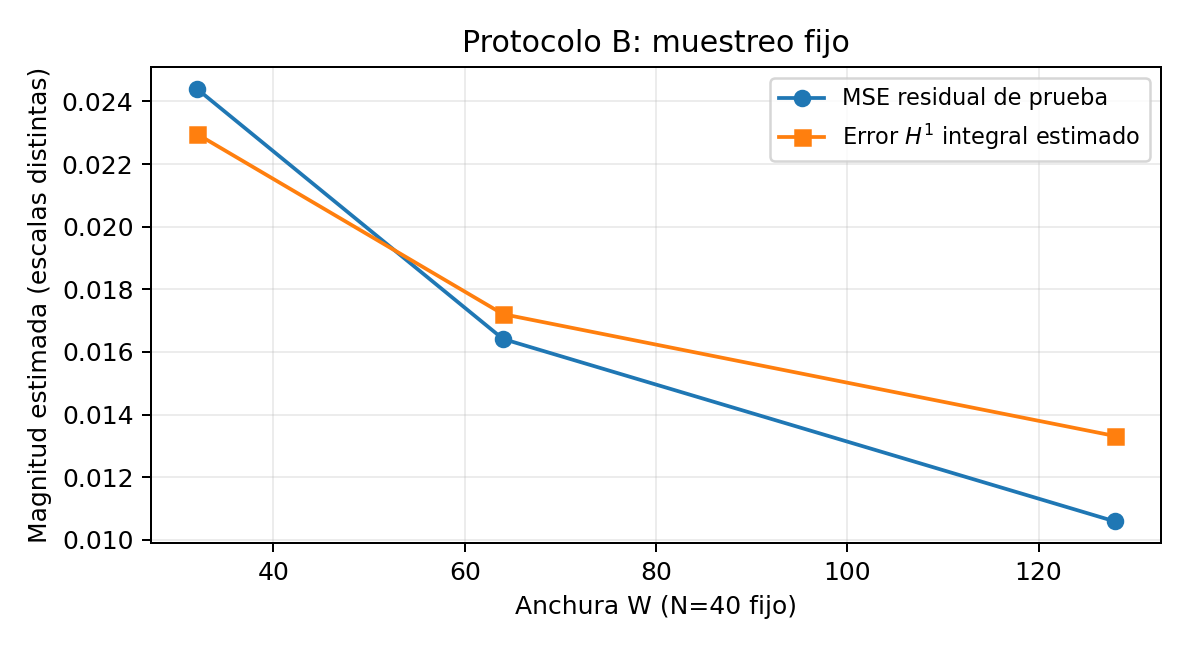
\includegraphics[width=0.82\linewidth]{imagenes/abc_B_anchuras.png}
\caption{Protocolo B con muestreo fijo: disminución de la MSE de prueba y del error integral $H^1$ estimado. Las magnitudes tienen definiciones diferentes; se presentan en los mismos ejes únicamente para mostrar sus tendencias.}
\label{fig:abc_B}
\end{figure}

\subsection{Protocolo C: escalamiento conjunto de puntos y anchura}

En C se consideraron los pares $(m_r,W)=(1521,64)$,
$(5476,128)$ y $(11881,192)$. La primera configuración reutiliza
\emph{exactamente} el entrenamiento B de $W=64$ y no se cuenta como
una nueva muestra independiente. Se conservaron dos semillas
por configuración. En la Tabla~\ref{tab:abc_escalamiento}
se muestran las medianas observadas.

\begin{table}[htbp]
\centering
\caption{Protocolo C: escalamiento conjunto. $\varepsilon_m$ es MSE residual empírica. La última columna es una seminorma residual estimada con 4800 pares, no una cota continua.}
\label{tab:abc_escalamiento}
\small
\begin{tabular}{rrrrrr}
\hline
$m_r$ & $W$ & $a_m^{\mathrm{int}}$ & $\varepsilon_m$ & $\varepsilon_m/a_m$ & H\"older (4800) \\
\hline
1521  & 64  & $1.232\times10^{-3}$ & 0.01645 & 13.35 & 2.312 \\
5476  & 128 & $4.714\times10^{-4}$ & 0.01355 & 28.74 & 2.053 \\
11881 & 192 & $2.637\times10^{-4}$ & 0.00890 & 33.76 & 1.943 \\
\hline
\end{tabular}
\end{table}

\begin{figure}[htbp]
\centering
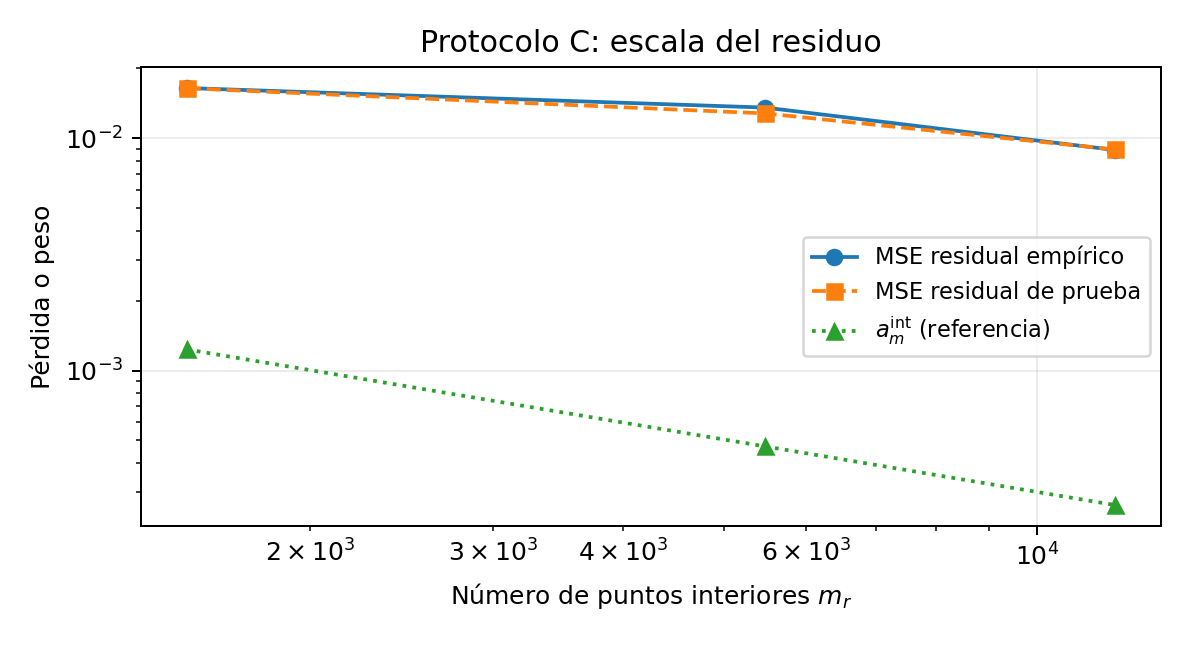
\includegraphics[width=0.77\linewidth]{imagenes/abc_C_escala.png}
\caption{Protocolo C: pérdidas residuales de entrenamiento y prueba en comparación con la escala teórica $a_m^{\mathrm{int}}$. El peso es una referencia analítica, no una curva ajustada a las pérdidas.}
\label{fig:abc_C_escala}
\end{figure}

\begin{figure}[htbp]
\centering
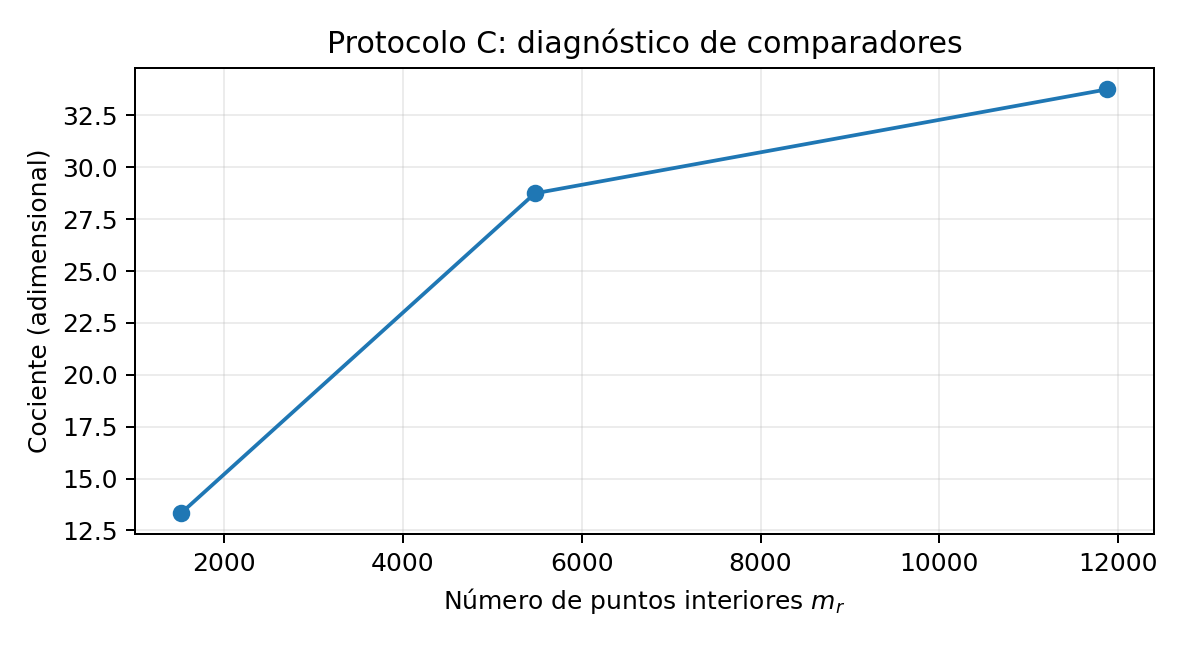
\includegraphics[width=0.77\linewidth]{imagenes/abc_C_cociente.png}
\caption{Cociente $\varepsilon_m/a_m^{\mathrm{int}}$ del protocolo C. Su crecimiento en las tres configuraciones no respalda todavía una cota uniforme para los comparadores entrenados.}
\label{fig:abc_C_cociente}
\end{figure}

El ajuste log--log \emph{puramente descriptivo y condicionado al
presupuesto fijo de optimización} de las tres medianas da
\[
 \varepsilon_m^{\mathrm{obs}} \propto m_r^{-0.284},
\]
frente a la escala suficiente $a_m^{\mathrm{int}}\asymp m_r^{-0.750}$.
Este contraste no estima una tasa intrínseca de aproximación de la
familia $\tanh$: en C también cambia la anchura y el entrenamiento
consta de 900 pasos Adam con lotes de 128 puntos y cuatro etapas
L--BFGS que utilizan subconjuntos de solo 512 puntos. Esos 512
puntos representan respectivamente 33.7\%, 9.3\% y 4.3\% de las
tres muestras interiores. Por tanto, el presupuesto efectivo de L--BFGS
cubre una fracción decreciente del conjunto de colocación. El primer
caso C reproduce B, no es una repetición independiente. Con tres
tamaños y dos semillas no se identifica una tasa asintótica ni se
demuestra que la condición falle para toda sucesión de redes.

La inspección con $1200$ y $4800$ pares muestra valores discretos
moderados del residuo, pero las estimaciones no son iguales.
La Figura~\ref{fig:abc_C_holder} permite apreciar la sensibilidad
a la densidad de evaluación; aumentar el número de pares no produce
por sí mismo una cota superior certificada.

\begin{figure}[htbp]
\centering
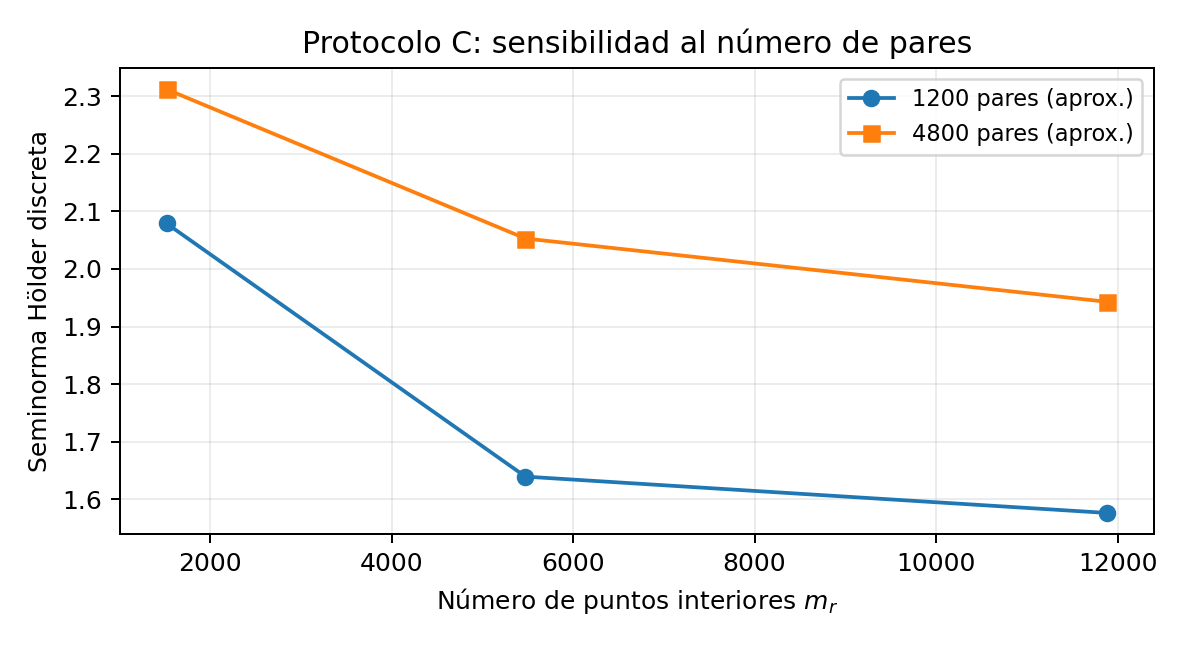
\includegraphics[width=0.77\linewidth]{imagenes/abc_C_holder_pares.png}
\caption{Estimaciones discretas de regularidad residual con dos presupuestos de pares. El supremo continuo no se calcula.}
\label{fig:abc_C_holder}
\end{figure}

\paragraph{Interpretación matemática.}
Los protocolos A--C respaldan que el refinamiento de la optimización
y el aumento de anchura, bajo las configuraciones ensayadas, reducen
los errores de prueba. Los valores discretos de regularidad no
presentan un crecimiento sistemático en el escalamiento C. Sin
embargo, la condición suficiente de la
Sección~\ref{sec:comparadores_aproximados} exige simultáneamente
control continuo de seminormas y una pérdida de comparador con
$\varepsilon_m=O(a_m)$; si se pretende extender la conclusión a
minimizadores aproximados, también una brecha
$\delta_m=O(a_m)$. El experimento no certifica ninguna de estas
propiedades asintóticas, ni la minimización global por Adam o L--BFGS.
El uso de muestras de entrenamiento aleatorias aproxima el protocolo
de muestreo de la teoría, pero no reemplaza la demostración probabilística.

\section{Comparación: elementos finitos (FEM), volúmenes finitos (FVM) y PINNs}
\label{sec:comparacion}

Finalmente, se realizó un estudio comparativo resolviendo la misma EDP de Poisson 2D utilizando tres enfoques numéricos distintos:
\begin{enumerate}
    \item \textbf{FEM:} Implementado mediante la librería \texttt{scikit-fem}~\cite{gustafsson2020scikitfem}.
    \item \textbf{FVM:} Implementado mediante la librería \texttt{FiPy}~\cite{guyer2009fipy}.
    \item \textbf{PINN:} Nuestra implementación en PyTorch~\cite{paszke2019pytorch}.
\end{enumerate}
El script comparativo itera sobre resoluciones de discretización para FEM/FVM y cantidades de puntos de colocación para la PINN. Estas cantidades no representan el mismo costo computacional; por ello, la gráfica debe entenderse como una comparación de error frente al parámetro de refinamiento de cada método, no como una comparación costo--precisión. El código del Apéndice A y el cuaderno computacional permiten reconstruir las tablas y figuras a partir de los solvers y entrenamientos registrados; los archivos de resultados conservados facilitan su trazabilidad. En esta comparación la PINN se resuelve con entrenamiento finito, de modo que la precisión observada depende del optimizador y de la semilla.

El barrido se ejecutó para $N\in\{10,20,30,40,60,80\}$; cada error se calculó sobre una cuadrícula común de $10\,201$ puntos. La PINN se entrenó durante $4\,000$ épocas por resolución, con distinta semilla en cada valor de $N$. La tabla permite cuantificar el comportamiento que se observa en la figura.

\begin{table}[htbp]
\centering
\caption{Errores relativos $L^2$ de los tres métodos en Poisson 2D.}
\label{tab:comparacion_fem_fvm}
\small
\begin{tabular}{rccc}
\hline
$N$ & FEM & FiPy (FVM) & PINN \\
\hline
$10$ & $3.891\times10^{-2}$ & $3.872\times10^{-2}$ & $1.261\times10^{-2}$ \\
$20$ & $9.743\times10^{-3}$ & $9.708\times10^{-3}$ & $1.176\times10^{-2}$ \\
$30$ & $4.325\times10^{-3}$ & $4.323\times10^{-3}$ & $1.584\times10^{-2}$ \\
$40$ & $2.433\times10^{-3}$ & $2.432\times10^{-3}$ & $1.372\times10^{-2}$ \\
$60$ & $1.081\times10^{-3}$ & $1.081\times10^{-3}$ & $1.373\times10^{-2}$ \\
$80$ & $6.082\times10^{-4}$ & $6.082\times10^{-4}$ & $1.094\times10^{-2}$ \\
\hline
\end{tabular}
\end{table}

\begin{figure}[h!]
    \centering
    \includegraphics[width=0.9\linewidth]{imagenes/comparacion_fem_fvm_pinn_reproducida.png}
    \caption{Comparación log--log de errores relativos $L^2$ para FEM, FVM y PINN en Poisson 2D, calculados sobre una cuadrícula común de evaluación. El parámetro de resolución $N$ no representa el mismo costo en los tres algoritmos.}
    \label{fig:comparison_methods}
\end{figure}

\begin{figure}[h!]
    \centering
    \includegraphics[width=0.92\linewidth]{imagenes/mapas_errores_fem_fvm_pinn.png}
    \caption{Distribución espacial del error absoluto de FEM, FiPy y PINN sobre el mismo conjunto de evaluación. La barra de colores compartida permite comparar magnitudes entre métodos.}
    \label{fig:mapas_errores_comparados}
\end{figure}

\begin{figure}[htbp]
\centering
\includegraphics[width=\linewidth]{imagenes/benchmark_mapas_error_escalas_independientes.png}
\caption{Errores puntuales para los tres métodos con escalas de color independientes. La figura permite examinar la estructura espacial de errores pequeños, pero no sirve para comparar magnitudes por color entre paneles; esa comparación corresponde a la Figura~\ref{fig:mapas_errores_comparados}.}
\label{fig:mapas_errores_escalas_independientes}
\end{figure}

\begin{figure}[htbp]
\centering
\includegraphics[width=0.86\linewidth]{imagenes/benchmark_poisson2d_error_vs_tiempo.png}
\caption{Error relativo $L^2$ frente a tiempo registrado para FEM, FVM y la PINN de referencia. Los tiempos corresponden a implementaciones y rutas de cómputo diferentes, no a un presupuesto igualado de recursos.}
\label{fig:comparacion_error_tiempo}
\end{figure}


\subsection*{Discusión comparativa}
\begin{itemize}
  \item \textbf{Exactitud.} FEM y FVM exhiben una disminución muy regular del error al refinar la discretización, aproximadamente proporcional a $N^{-2}$ en el rango estudiado. En la ejecución $N=10$ la PINN registra el menor error de los tres métodos, pero una sola semilla no autoriza atribuir una ventaja sistemática a la formulación. El error PINN oscila, en parte porque la semilla de entrenamiento cambia con $N$.
  \item \textbf{Costo.} Para $N=80$ se registraron $3.12$ s (FEM), $0.076$ s (FVM) y $23.68$ s (PINN) en las implementaciones utilizadas. Son tiempos de la ejecución concreta, no una comparación normalizada de hardware ni de costo de obtención de una misma exactitud: la PINN usó aceleración CUDA y los solvers clásicos siguieron rutas distintas de cómputo.
  \item \textbf{Comparabilidad.} El número de celdas, los grados de libertad de FEM/FVM, los parámetros de la red y las evaluaciones del residuo son recursos diferentes. Una comparación costo--precisión completa debe reportar tiempo de pared, memoria y número de parámetros o grados de libertad.
  \item \textbf{Integración de datos.} La PINN incorpora observaciones mediante un término adicional de pérdida. Esta es una diferencia de formulación útil, pero el capítulo no compara problemas inversos ni métodos clásicos de asimilación de datos.
\end{itemize}

\section*{Conclusión del capítulo}

Los ejemplos de regresión, crecimiento logístico y Poisson 1D permiten seguir el tránsito desde el ajuste de una red hasta la minimización de residuos diferenciales. La separación de componentes de pérdida identifica restricciones dominantes durante el entrenamiento, pero no equivale a una separación del error de solución. La comparación exploratoria de regularizadores 1D no permite derivar tasas asintóticas.

La reproducción bibliográfica con Dirichlet débil para $u^*(x)=\tanh(x)$ muestra una reducción cualitativa del error al ampliar la muestra. El segundo problema, con solución altamente oscilatoria y Dirichlet fuerte, no reproduce la tendencia decreciente publicada. Una revisión de la función objetivo corrigió el peso regularizador y un diagnóstico posterior mostró respuestas distintas al uso de minilotes en PINN y LIPR. La causa de la discrepancia no se reduce a un solo elemento de protocolo y sigue abierta.

El diagnóstico H\"older ilustra la importancia de la regularidad del operador y la cobertura de los puntos de colocación, pero sus máximos discretos no constituyen certificados del supremo continuo. En dos dimensiones, la evaluación conjunta de los residuos y errores en una malla independiente aporta evidencia sobre la separación entre pérdida empírica y comportamiento fuera de la muestra. En particular, con Dirichlet fuerte y $N=12$, la pérdida residual media cuadrática de prueba supera en torno a $576$ veces a la de entrenamiento.

El barrido principal de Poisson 2D comprende cuatro resoluciones, tres semillas y dos tratamientos de frontera. La parametrización fuerte produjo, en $N=75$, una mediana del error relativo $L^2$ unas $35.6$ veces menor que la versión penalizada, y un error relativo $H^1$ unas $25.7$ veces menor. El menor error requirió mayor tiempo de entrenamiento y mostró estabilización en las resoluciones más altas. Estos resultados constituyen evidencia computacional en un régimen finito, no una prueba de las hipótesis de convergencia asintótica del Capítulo~\ref{chap:convergencia}.

El estudio de comparadores aproximados con redes $\tanh$ distingue optimización, anchura y escalamiento de muestreo. En el protocolo C, la MSE residual disminuye mientras el cociente $\varepsilon_m/a_m^{\mathrm{int}}$ crece entre las tres escalas consideradas. En consecuencia, las observaciones no verifican la tasa suficiente del Capítulo~\ref{chap:convergencia}; tampoco la contradicen como afirmación asintótica bajo hipótesis adicionales.

En la comparación exploratoria de FEM, FVM y PINN, los métodos clásicos presentan un error que decrece de modo regular bajo refinamiento. El entrenamiento PINN del benchmark original no tiene un presupuesto ni un número de semillas que permitan juicios generales de superioridad. Las figuras con escalas comunes e independientes distinguen comparación de magnitudes de inspección espacial, mientras que la figura error--tiempo documenta únicamente el costo observado en el entorno registrado.
